\chapter{Analysis} \label{chapter-analysis}
% Get banks 'We are the biggest innovators in history quote'
%``Financial engineering has created a rentier class, a modern feudal system, and the biggest beneficiaries of all that extra debt have been the bankers.'' Times, Sunday Times (2016) 

In the base model, we only allow the radius of the city to change, and not the density and firm hiring behaviour.\footnote{Complex city form, density patterns, and alternative hiring patterns, can be easily incorporated in the computation model. We expect that they would not significantly affect our conclusions.}  
% model rules, and individual 
%and the job search process. 
% In practice, many other factors impinge on these choices. %additional decision factors, agents, driving variable, and \gls{stochastic} elements enter the model. 
---


\section{Class}
We use the concept of \gls{class}  to explore the consequences  of financialization in the housing market. The term class was  used  by classical and Marxist economists to refer to patterns in the ownership of productive assets.\footnote{ Erik Olin Wright summarizes the approach common to classical and Marxist analysts:  ``The fundamental contrast in capitalist societies, for example, is between owners of means of production and owners of labor power, since ``owning'' is a description of rights and powers with respect to a resource deployed in production.''\cite{wrightAlternativeFoundationsClass2002}} Those who had only their labour to sell were \gls{working class}. Those who lived off the rents from the land they owned were \glspl{landowner}. Those who captured the surplus from industrial production because they owned the capital stock were capitalists, and those who lived off the the income from property or money lent were \glspl{rentier}.\footnote{The term rentier is used variously. It is applied to people living off the income from already acquired wealth, and applies, for example to pensioners.  In ``rentier capitalism''  it is a noun meaning ``a business model in which ownership of key types of scarce assets-such as land, intellectual property, natural resources, or digital platforms-is all-important and dominated by a few unfathomably wealthy companies and individuals called rentiers. Financialization } 

\begin{table}[!ht]
    \begin{centering}
\begin{tabular}{lcccccc}\small
  
    & \multicolumn{6}{c}{Means of Production}\\   \cline{2-7}
     &labour &talent & education& land & \multicolumn{2}{c}{capital} \\ \cline{6-7}
     &       &       &          &       &real   &financial  \\ 
     \hline
      \multicolumn{7}{c}{working classes}\\
simple& X   &       &         &         &       &\\
gifted& X   &    X  &         &         &       &\\
professional& X   &       &    X   &         &       &\\\hline
& \multicolumn{6}{c}{middle classes}\\  
   \multicolumn{7}{c}{lower}\\
Middle  & X   & * & X  & +&  + & +\\
classes & X   & X & *  & + & + & +\\\hline

 & \multicolumn{6}{c}{upper (\textit{working owners})}\\
% \multicolumn{7}{c}{}\\
landowner & X  &   *   & * &   X   &   *  & * \\
capitalist& X  &   *   & * &   *   &   X &  *\\
rentier   & X  &   *   & * &   *   &   * & X\\\hline

&&&& \multicolumn{3}{c}{pure owners}\\
landowner  &   &  & &   X  &       &\\
capitalist &   &  &  &     & X  &\\
rentier    &   &  &  &     &   & X\\ \hline
\end{tabular}
\end{centering}
\vspace{.25cm}

``\textbf{X}'' and “\textbf{+}” together indicate class identification

``\textbf{+}'' signs in a given row indicates `` at least one of these is included.''

\noindent``\textbf{ * }'' signs in a given row indicates `` may be included.''
\caption{Classes by asset ownership}
\label{table-classes}
\end{table}
% \usepackage{xcolor}
% \usepackage{nicematrix}
% \begin{document}
% \begin{NiceTabular}{lllllll}
% \CodeBefore
%   \rectanglecolor{blue!20}{2-2}{6-6}
%   \cellcolor{green!20}{7-7}
% \Body
%   & 1 & 2 & 3 & 4 & 5 & 6\\
% 1 & 1 & 1 & 1 & 1 & 1 & 0\\
% 
% 6 & 0 & 0 & 0 & 0 & 0 & 1\\
% \end{NiceTabular}
% \end{document}


This basic classification is too simple, of course. To describe a real society more fully, it has to be completed with a variety of sub-classes and intermediate classes. Table~\ref{table-classes} illustrates one approach based on Roemer's  \textit{A general theory of exploitation and class} \cite{roemerGeneralTheoryExploitation1982}. Variations in assets generate distinct professions, identities and alliances far more complex than a simpler version would suggest. The model allows for mobility between classes of the sort we suggest is occurring as a result of financialization of the housing market.

Workers, for example, who sell not just their labour, but also their talents and/or the services of their education will earn more as a rule and live better. Talents may include native skill in carpentry or coding, or beauty. Education includes the long apprenticeship of talented artists and  trades training as well as postsecondary education, management experience, or experience on wall street. It is worth noting that education is achieved by investment and is a capital asset, while talent is a gift of nature like land. 

The middle classes are especially complex because of the variety of assets individuals may own. The traditional shop owner, for example, often described as a member of the \gls{petite bourgeoisie}, may work in his own a shop and with his equipment and enjoy a relatively comfortable income, but still  need to apply his own labour. The professional classes have skills as a result of their investments in learning their profession. the market value of their human capital may be increased by professional organizations that restrict entry to the profession, and augmented by social capital.  Despite the similarity between the craft trades and the professional trades, the latter generally have greater social status. Consideration of social  further complicates discussions of class.

One of our goals is  to show how financialization of the housing market drives change in the class mix within cities using this asset-based understanding of class.





we could also think of location as among them





\section{Investment amplifies the problem of financialization}
\section{financialization amplifies the problem of housing shortages }

\begin{enumerate}
    \item to model set a low alternative $i$ and then put a dial on the amount of K in any period (this is friction)
    \item Vary individual costs of capital - the function that raises the rate for the poorer buyers can be made steeper.
    \item How do we make $\dot p$ more volatile - this feeds into developer decisions
\end{enumerate}

This will accelerate tenantization.

\subsubsection{holding property for later development}

\begin{enumerate}
    \item We need a density function. Redevelopment is increasing density. Unit size (land per unit) is constrained by a utility function  (but only for newcomers, I think.) 
    \item with a density choice increasing density can be delayed.
    \item you could even set a hard boundary on the city and just explore density. 
    \item We need a way to increase population pressure. (maybe just amplify the wage
\end{enumerate}
If it's not a supply problem
Leaning into rental removes a key piece of how we've build the model


Would get pieces held off the model.
get units held off the market.


Model to hold the developer.. 
Need a desnity function, go to a different density..
look to see when it's better to wait to invest in increasing density.

\section{Financialization: Implications of the bidding rule}

There are some implications of the financialization mechanism:
\begin{enumerate}
\item A large $m$ magnifies the return. (The downpayment is smaller as a fraction of the price, increasing the investor's leverage). 
Given the  common rule that mortgage payments cannot exceed some fraction of disposable income, the wealthy will be able to borrow larger amounts and at lower interest rates than the less wealthy. At any distance from the centre they will be able to make a higher bid.

\item A lower mortgage interest rate increases the return by lowering interest payments. The cost of capital is known to differ for rich and poor.  The wealthy can generally borrow  at lower interest rates than the less wealthy. 

\item A lower discount rate $\delta$ reduces the subjective rate of return.  Poverty in assets and cash liquidity constraints are correlated with higher rates of time preference  \cite{carvalhoPovertyTimePreference2010}\cite{holdenPovertyMarketImperfections1998}. If agents discount at their borrowing rate, wealthier agents may have a lower subjective rate of time preference and therefore value properties more highly. 

\item Higher expected price appreciation increases the attractiveness of an investment. Financial corporations and the wealthy are likely to have better price forecasts than  the occasional home buyer.

\item Higher rents make the unit more profitable. Higher expected  rents may result from expecting greater price appreciation  leading to raising rents for tenants. Lower discount rates may give future rent increases greater present value.

\item Lower maintenance costs increase profits. There may be scale economies in the maintenance  of rented housing. 

\item Lower tax rates decrease holding costs and increase the value of the investment. There may be opportunities to shelter income with land held for investment (speculative) purposes. Tax treatment of income and capital gains as well as interest deductibility may also provide advantyages for institutional buyers and investors.%\footnote{Case and Schiller \cite{LOST_CaseandSchiller} observe that (source?) `` ... increases in real per capita income all are positively related to excess returns or price changes over the subsequent year.''} 
\end{enumerate}

Some  of these conditions (1-3) hold generally for wealthier actors. Others (4-7) may be available only to institutional investors.  Financial corporations in particular may have advantages relative to individual investors, making it  reasonable to expect that financial corporations increasingly dominate urban land 
markets.\footnote{Fr\'ed\'erick Demers \cite{demersModellingForecastingHousing2005} found that the response of housing investment to interest rates has become more pronounced over time. This suggests a rising share of financial investors relative to buyers focused on housing services. Case and Schiller \cite{caseThereBubbleHousing2003} observe that `` ... increases in real per capita income all are positively related to excess returns or price changes over the subsequent year.''}  

Since interest rates are lower for those with higher wealth, the analysis implies, consistent with the empirical evidence, that net returns for investment are increasing with wealth. Large wealth holders will get higher expected and actual rates of return on land than those with lower wealth holdings. Managers of large pools of capital will have an even greater   advantage. Overall, Equation~\ref{eqn-bid-price} implies  sales generally go to the richest participant.
 
%  \footnote{Case and Schiller \cite{LOST_CaseandSchiller} observe that (source?) 
%  `` ... increases in real per capita income all are positively related to excess returns or price changes over the subsequent year.''} 

% The conclusion that we draw from the analysis above is that  financialization of urban housing benefits a rentier class of urban landholders. There is evidence that it benefits a globally distributed class of rentiers.  



\section{Financialization as system change} \label{section-system}
We established that, at least in theory,  financial institutions and the wealthy are likely to own increasing shares of the housing stock. the theoretical conclusions is consistent with what has already happened in the Canadian Housing market. Recent data from Statistics Canada \cite{fontaineResidentialRealEstate2023} suggests people who own more than one property in Ontario make up more than 25\% of buyers in the province. (The proportion of investors among owners varied from 20.2\% in Ontario to 31.5\% in Nova Scotia.)
Just under one in five properties overall was used as an investment.
In Ontario 41.9\% of condominium apartments are investment properties \cite{statisticscanadaBuyRentHousing2022}.

The immediate social implications are fairly obvious. As Statistics Canada points out, these trends might limit the number of properties available to buyers who intend to use it as a primary place of residence  \cite{fontaineResidentialRealEstate2023}. Statistics Canada reports that latest census release, two-thirds of Canadians owned a home in 2021, down from a peak of 69 per cent a decade earlier. The decline is was higher for younger members of the population. 

When the homeownership rate goes down, the rental rate goes up. The 2021 Canadian Housing Survey reported that the number of renter households increased  at over twice the pace of owner households, pushing down the homeownership rate in Canada. If the trends continue, Urban Canada will gradually change from a society dominated by homeowners to a predominantly tenant society. Since wealthier buyers are advantaged in the market, the younger and poorer parts of the community will be increasingly excluded from ownership. Financialization will increase income and asset inequality in cities.

Combined with rising housing prices the effect will be to squeeze lower-wage households closer to what we have termed to subsistence level and make it harder for low-wage workers to live in the city. The city requires low-wage workers for many of the services, so labour shortages are a possibility. Labour shortages will squeeze some activities out of the city and are likely to reduce productivity. Labour shortages may push up wages, but in rental markets, landlords can capture much of any increase in wages. 

The incentive structure in our model was derived purely from the point of view of an individual investor. Examination shows that investment incentives favour the wealthy and institutional buyers, but that does not necessarily imply that the process of financialization will drive social transformations. Individual choices are at most  a link in the chain. Modelling  allows us to identify which parameters are most influential. 

A question that is especially important is whether the process of financialization and tenentization our micro model suggests is reversible:  high levels of home ownership we have seen throughout the 20$^{th}$ century, as Purdy \cite{purdyPropertyOwningDemocracyHome1993} suggests, may be ``a transitory phenomenon of the 20th century.''

% .#https://www.jstor.org/stable/j.ctt80wdt Housing the North American City
% MICHAEL DOUCET
% JOHN WEAVER
% Copyright Date: 1991
% Published by: McGill-Queen's University Press
% Pages: 608
% https://www.jstor.org/stable/j.ctt80wdt

 %how financialization might affect  the housing market as a system and some consequences for society in general. At that point we can introduce our specific hypotheses and how we intend to test them.
%***E IF YOU WANT TO INTRODUCE ANEW USE OF THE TERM, CONTEXTUALIZE IN TERMS OF HOW YOU ARE USING THE WORD. IS THIS AN EXTENSION OF HOW YOU USE IT? THIS SEEMS RELATED TO THE MACRO VERSION YOU MENTION ABOVE. MAKE THE RELATIONSHIP CLEAR. I ALSO WONDER IF THIS WOULD BE USEFUL TO MOVE UP. IT FEELS LIKE IT MAKE BELONG WITH THE BROADER CONTEXT AT TEH BEGINNING OF THE CHAPTER? GOOD IDEA I will try it

*e tHIS IS CLEAR BUT COULD BE HELPED BY RESTATING HOW THEY MOVE IT ONTO FINANCIAL MARKETS. JUST A QUICK SUMMARY STATEMENT OF HOW THEY ARE FINACIALIZATION. %EVEN JUST something like... They put the ownership of housing onto financial markets. just to keep us oriented in what we are talkign about.

*E I FEEL LIKE THERE IS SOMETHING MISSING BETWEEN THESE TWO PARGRAPHS. %PERHAPS JUST FLESHING OUT WHAT FINANCIALIZATION LOOKS LIKE TECHNICALLY. MAYBE ALSO INSTRODUCE POSIBLE EFFECTS... LIKE EVEN JUST INTRODUCE THEM AS QUESTIONS? IT'S BEEN SUGGESTED OR SHOWN THAT ITS CONTRIBUTING TO THE HOUSING CRISIS. tHIS WOULD ALSO BE A GOOD PLACE TO EXAPLIN WHAT YOU MEAN BY ``aS SYSTEMS CHANGE... BECAUSE i THINK THAT IS A BIG PART OF WHY YOU SAY NEXT THAT IT NEEDS TO BE UNDERSTOOD... BECAUSE IT HAS SUC BROAD EFFECTS

We need to understand the economics of financialization.
% \section{Literature on theory and evidence} % PROVIDE EVIDENCE 	mention theories?
There is substantial evidence that the financialization of urban housing is underway in Canadian cities..

Two questions arise when we observe the growing participation of global capital in the urban housing system: 
\begin{enumerate}
\item How far will the financialization of urban land go? 
\item That are the implications for the urban economy and the welfare of the urban population? 
\end{enumerate}

We can demonstrate that in the absence of policy interventions, differential access to finance capital ensures that capital owners acquire an increasing share of urban land % over time
and therefore capture the growing land rents from urban productivity growth. 

With this insight, growing wealth inequality emerges within a simple, widely accepted model of the urban land market. In the limit, urban residents are tenants, and new residents without capital no longer receive any of the increases in rents arising from the growing productivity of the city. 

%The first question, therefore, is reduced to which capital holders will increase their share of urban land and whether there is any reason to expect the process of financialization process to stop or reverse itself.

% \section{The incentives for financialization}
%Instead, drawing on the ideas of Jane Jacobs, Lucas proposes the city as the unit of analysis. Lucas, Robert (1990), ``Why Doesn't Capital Flow from Rich to Poor Countries?,'' American Economic Review Papers and Proceedings v. 80, no. 2 (May) pp. 92-96.  
%Jacobs, Jane  (1969), The Economy of Cities (New York: Random House).  
% The Death and Life of Great American Cities \cite{jacobsDeathLifeGreat1961}

MOVE The mortgage share and interest rate are functions of the agents wealth %Both the  share of the price  that can be mortgaged, $m$, and the interest rate and the interest rate paid, $r$, are functions of the agent's wealth. 
The discounting factor may be correlated with wealth as well. 

%%%%%%%%  VVVVVVVVVVVVVVVVVVVVVVV   This section May 18 to cut?  V
%%%%%%%%  ^^^^^^^^^^^^^^^^^^^^^^^   This section May 18 to cut?  V
% TODO - add interest rate discussion - (borrowing rates drive land prices up, even if there is no development or improvements, simply because it makes it worth a larger--the effect of low rates, especially for institutional actors have driven a large effect)
%\begin{enumerate}
%
%\item  the buyer and seller calculate the value of the property  differently. 
%
%\item  the  buyer and seller may have different expectations of the path of prices and therefore the stream of rents.
%%There are two standard ways that expectations are modeled
%%	\begin{enumerate}
%%	\item \textbf{Adaptive expectations.} Expectations are largely based on what has happened in the past. 
%%	Under normal conditions most people  have relatively weak incentive to get forecasts about inflation correct and lack the resources and time to purchase expert advice. 
%%	Recent price trends are easily available and likely to be the main source of  information.
%%	\item     \textbf{Rational expectations.} Expectations are based on a model of the future economy. 
%%International investors and banks employ economists and other experts to  forecast prices, exchange rates, and trends in the economy.
%%	\end{enumerate} 
%\end{enumerate}
% Why would  discount rates differ between identical workers? Buyers and sellers are not identical in wealth, . 
%%We could implement the first  explanation either by generating expectational errors based on functional class or wealth. 


\section{Distributional consequences of the analysis}
The analysis in this dissertation makes clear that in addition to distributional consequences, the housing crisis has productivity impacts. Specifically, the analysis in this thesis concludes that, given the ongoing financialization of the housing market:

\begin{enumerate}
\item the financial system will eventually extract all net urban land rents through investment in urban property
\item housing accessibility will become increasingly challenging for disadvantaged groups
\item housing will be largely eliminated as a saving mechanism and asset fr middle income Canadians,  resulting in a systematic decline in the `middle class'
\item that the quality of urban life will decline
\item the economic growth and development of cities is threatened by this financialization
\end{enumerate}

RESILIENCE AND INTERST RATES..

% These implications should be considered in policy.



\section{Resilience}
Historically low interest rates, and financial crises, have been a primary driver of rapid inflows of financial capital, accelerating the process, which raises the question of what will happen as interest rates rise. The analysis suggests however that there is hysteresis, that both the economic upswing and the downswing pull wealth out of communities, like a kind of ratchet or peristaltic pump. We analyze and model these dynamics in the resilience Chapter, %Chapter~\ref{chapter-resilience}

The model gives a resilience result which is that shared wealth through housing is not resilience.

It can also be used with a driven version of the model to show that the model pumps wealth out on the upswing and on the downswing - like a kind if ratchet.


\section{Resilience background}

This section explores the resilience dynamics of distribution of wealth within a class of market models.  

Using a systems design approach and looking at resilience measures and alternative regimes gives insights into patterns of distribution and how that shapes wealth. 

The two significant concepts of resilience for this work are the relationship between distinct alternative regimes and patterns of cycling within a single regime. 

\section{What is resilience and how is it connected to this work}

Resilience is a concept that has to with the way in which a system resists disturbance or maintains identity through disturbance. The concept has emerged independently with different, but related definitions in various fields. 
There are a class of systems that this idea of resilience should be applicable or illuminating for, however the concepts and measures that exist already are ill-suited to the dynamics of the system. 
The work in this thesis draws from the measures from existing measures and concepts of resilience from various discipline to evolve a measure that can apply to this other class of systems. 

Shaping this c
ore broadly applicable concept that 
We can approach change in various systems using technical tools that are transferable. 
The concept 

\section{Resilience in engineering}

In engineering, Resilience is defined as the return properties of a system. 
It is the measures relating to how a system comes back to its stable equilibrium or stable state. For example if you push a branch on a tree, it will oscillate and settle back to its resting position. 

Stability properties are important in engineering because engineers are responsible for signing off the performance of system, whether the the system is a bridge or a chemical reactant or an electrical circuit. Stability is an aspect of the system’s behaviour. The engineer needs measures to predict the stability of the system when it's perturbed. (Specific) 

Engineering resilience is distinct from the failure zones or the threshold of failure - for example the level of force/weight or number of stress cycles that would be required to collapse a bridge. While those measures pertain the thresholds beyond which the system would fail, resilience is about describing how the system recovers from perturbations that do not break it. 

The primary measure is how long the system takes to return to its equilibrium, i.e. the return time. (Equation) There are seven measures, listed in table XYZ that pertain to return to equilibrium properties.  (Table)

There is some variation in the use of the concept in specific disciplines of Engineering. For example, in transport engineering it has something to do with traffic flow.

\section{Resilience in ecology}

In Ecology resilience is defined as the way in which systems maintain identity through transformations. 

In engineering, the concept of resilience centres on the idea of a single equilibrium. If the system is not disturbed, it will stay at equilibrium and the resilience measures account for the system’s return to this equilibrium. In the ecology, on the other hand, instead of a single equilibrium the underlying pattern of the system has a dynamic structure. For example the ecosystem of a forest contains ongoing cycles of life and death and evolving patterns and interactions and yet sustains its identity as a forest. 

An ecosystem can experience big shocks or disturbances without losing its basic identity. For example, there can be drought, floods, fire, species loss, etc and the forest can recover and continue to be a forest. 
((The forest can regrow, one species might replace another and the forest changes but it doesn’t necessarily stop being a forest.)) But some disturbances can tip the ecosystem over into a different pattern of functioning. For example if the land is cleared and animals come into to graze the seedling trees so that they do not grow back, the forest can transition to a grassland ecosystem. Or if the region becomes dry enough, the forest can transition to become a desert. 

In ecology these alternative patterns of a system that may be identified as a forest, grassland, or desert are called regimes. In Ecological resilience studies, this concept of regimes replaces the simpler idea of equilibrium, differing both because the underlying pattern is more complex and because there are multiple regimes that the ecosystem of the same land can shift between. 

Part of what resilience in ecology is getting at, then, is what kind and how big the disruption can be before the ecosystem becomes a different kind of ecosystem. Resilience measures describe the properties of these distinct regimes and the relations between them. The most common measure is the size of the perturbation the system can withstand without transitioning into an alternative pattern of functioning or regime.  

This approach to resilience was introduced by C.S. Holling with his 1973 paper on a Spruce Budworm model of a forest ecosystem. In this paper he argued that there was an evolving interrelationship/feedback cycle between Spruce growth/regrowth and the population of Spruce Budworms that eat them. This interaction drove ongoing cycles of forest recovery and collapse. 

Holling’s work established the concept of these kinds of cycled and alternative regimes in ecosystems. Subsequent work by Marten Scheffer in lake eutrophication validated that alternative regimes appear in ecosystems in the real world. Now there is a database tracking thresholds and regime shifts in ecological systems with over a hundred entries showing its common.  ([https://www.resalliance.org/thresholds-db](https://www.resalliance.org/thresholds-db)) 

In ecology, this idea of resilience has evolved into a dynamic concept that is important in climate change science and ecological conservation. Resilience measures show how a system maintains identity through change by measuring the relationship between regimes, that is how close a system is to transitioning to a different regime or pattern of functioning. Thus the concept of ecological resilience and alternate regimes give tools to understand what is possible for an ecosystem. This give insight both into how ecosystems can be preserved but also what happens when they transform. 


\section{Resilience in social systems}

The ecological concept of Resilience has since been applied widely to various systems across disciplines (*INSERT EXAMPLES*). Frances Westley applies Holling’s idea of alternative regimes to social systems as the basis for a theory of social innovation. 

Westley defines social innovation as “a change in the routines, resource flows, authority flows or beliefs in any social system.” According to Westley “a successful social innovation also has durability and broad impact.” 
Her studies in social innovation focus on how individuals, groups, or institutions are able to shift social systems to achieve certain goals. 

Westley’s research question is how social systems transform. This frame differs from the majority of resilience work in engineering and ecology because the focus there tends to be on maintaining the integrity of the system, whereas Westley’s work is focused on how to move between regimes. 

For example, in the Great Bear Rainforest in British Columbia in the late 1990’s (??) clearcutting for pulp and paper was threatening some of the last old old growth forests in the region and disrupting the lives of people who depended on them. Over years of unchecked logging combined with a history of land appropriation, there was ongoing local resistance. In 199X images of the devastation spread through international media and led to a boycott of paper products from clearcutting. This moment of crisis brought the forestry industry to the table. After a carefully structured process of conversation and engagement between community organizers, political leaders, and industry they put the Great Bear Rainforest under Indigenous community control. 

This change in governance structure can be understood social system that can be understood as a regime change because there were a set of patterns and feedbacks holding the old system in place and and there new set of patterns and feedbacks holding the new system in place. Each regime has a distinct pattern of functioning or identity. 

The idea of resilience in social innovation illuminates how the patterns of different regimes structure the social systems. What is different about the two regime in the case of the Great Bear Rainforest is the distribution of the flow of money and power - or the the language of social innovation, resources and authority. This changed the routines and habits of the people making up the social system as they became more directly involved in managing the forest. The result is that the ancient Great Bear Rainforest survived. 

The study of resilience within social innovation looks at how actors within  systems play a role in shaping transformation of interconnected social-ecological systems. Westley specifically studies individuals, groups, or institutions who have the intention to shift social systems to achieve certain goals. This means that there is a directed strategic nature to the agents. This is illustrated by the case of the Great Bear Rainforest by the different stakeholders from industry, community and governance who are are all actively working to achieve specific goals. However none of these actors are outside outside the system. Even those with power cannot completely control the system. Their efforts interact with the actions of others and the broader context of the whole

Social systems are dynamic. There is no fixed equilibrium and yet they have clusters of properties that persist and can prove difficult to change. These patterns with distinct identities are described in social innovation theory as regimes. These patterns can pertain to various feature, from the routines that structure interactions to resource flows within the system. In the example of the Great Bear Rainforest, under the previous system the resources and money flowed out of the community and decisions were made by distant corporations. The shift in governance structurally affected both the ecosystem and the culture of the communities. When they shifted to community governance, the emphasis shifted away from extraction and toward investing and building the forest and the community. (ADD CONCRETE DETAILS/NUMBERS?) 

Sometimes people can achieve their goals and sometimes they do not and it depend on both what they do and the state of the system. In her grounded theory work studying people who have attempted and succeeded in changing systems, Westley observed that sometimes there are moments of opportunity that make shifts in the system possible.  In the rainforest example, there were years of Indigenous organizing and building an environmental movement. 
The change became possible at a particular moment when commodity prices were placing pressure on the industry and coordination between local and national environmentalists resulting in international boycotts of pulp and paper products from clearcut forest, particularly across Europe. The indigenous organizers were able to achieve more in this moment of opportunity.

According to Westley a successful social innovation also “has durability and broad impact.” This is a description of the change but it also illuminates how the resilience concept of regimes is useful. One feature of systems is that a set of feedback loops will hold patterns of interactions, resources flows, etc in place. Many changes simply die out.  The changes that last do so because they change the flows and dynamics in ways that are held in place by new feedback loops.  Social Innovation theorists have used the concept of regimes to explain this phenomena. If the system state is perturbed enough another set of patterns can come to dominate.  (MAKE SURE THESE TERMS ALIGN WITH THE PRECISE TERMINOLOGY USED LATER) In the example, after the shift to the community governance that became self-reinforcing as different feedback loops emerged to structure the building of relationships and institutional structures, community habits, networks of support, and resource flows. 

\section{Role of this thesis}

What has been articulated in Social innovation theory is a story of how feedback loops hold the patterns in place  and how systems can switch between sets of patterns. Westley and others have applied the concept of resilience as an explanatory framework, rather than as a a precise mathematical statement. 
The thesis seeks to operationalize these concepts within a formal model in the context of social systems. 


- By operationalizing into this model, we can patterns in how systems shift between regimes. Specifically in this thesis the models show where in the systems there are opportunities - ie the system is more vulnerable or -open to change. 
- In practice regimes change can move you into a more or less desired state. Here I focus on opportunities and interventions. 
- Inventions are…
- By looking at where the system has opportunity to change this work illuminates how actors might be able to identify opportunities for regime change. 
- 











he analysis has been applied conceptually, rather than as a precise mathematical statement. Thus far, in the study of social innovation 

Routines, resource authority flow and beliefs. 

International concern
Boycotts 
Political movement

Effective local movement established an indigenously led sustainable forest and tenure
It 



Community leaders were able to establish a 




Social innovation involves interventions or actions 




She studies I

Change in technology and demand for wood. 

For example, she looks at how various countries responded to the AIDS crisis and how activists in certain shaped 

There’s a debate about how systems transform. 
Impersonal forces of history like the development of agriculture
She’s studying the phenomena of change in order to inform 
The research is about how people try to change the word. 

(ie. a system consisting of different interconnected entities such as  individuals, groups, and institutions relating to each other and forming a whole.)

An interdependence of a social and cultural element 

Series of interrelationships between individuals and groups and institutions forming a whole. 



% [[adaptive cycle]]


\section{Resilience and class}

(TODO: introduce the idea of class in the resilience section, and link it to the resilience of the wealth trajectories.)  
reversibility/hysteresis, and how class is treated in the literature.
Three spatially segregated ``\glspl{class}.'' Capitalists live in some spaceless utopia,  Urban workers who commute and earn wages in the urban commuter-shed, and  rural residents and landowners who may choose to move to the city. There may be a band surrounding the city or persons who do not commute but enjoy urban consumption amenities. 
a fourth class, the urban tenant. 
Developed in Chapter~\ref{chapter-model} on modelling.

The model is we employ consistent with the theories of Ricardo and Henry George in locating the ground of urban exploitation and class in the capacity to extract social surplus through land ownership, and differs from the standard Marxian analysis in its reliance on access to financial capital rather than control of productive physical capital. The paper concludes that given existing land ownership patterns which encourage speculative investment, housing prices must rise and income inequality must increase. 

In the classical language, someone is exploited if someone else gets a share of the value of their labour. %(REPLACE WITH MORE PRECISE DESCRIPTION). 
 Employers capture a share of the value of workers' labour, so they exploit workers under this definition.
Those who own land early in a growing city are also capture a share of everybody's production. Since they capture a share of the productivity of others working in the city, through the rents, they are also exploiters, they form a kind of hybrid class. %Rents could be captured directly through renting out the property after they retire away from the city,  or by selling the property at a higher value than they bought it. 



\section{Differential transportation costs}
 Urbanists agree that before the railroad and the automobile, the extent of a city was roughly determined by how far a person could walk in about an hour. The time and effort cost of transportation determined the size of cities. 
 
 It also affected the distribution of the classes within the city. When everyone walked, the  wealthy may have valued their time more than the poor. In terms of the model, the willingness to pay for the rich would begin higher than it would for the poor, but would descend more rapidly with distance

\begin{center}
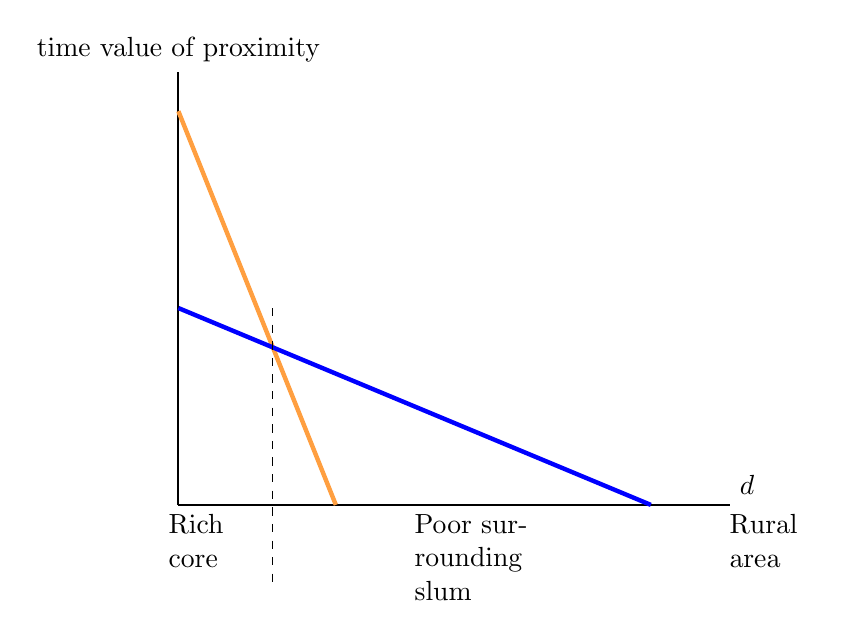
\begin{tikzpicture}[scale=1]

    \draw[thick](0,0)--(0,5.5)node[above]{time  value of proximity}; %Y
\draw[thick](0,0)--(7,0)node[above right]{$d$}; %X

\draw[ultra thick, orange!75](0,5)--(2,0);
\draw[ultra thick, blue](0,2.5)--(6,0);
% \node[draw=white, fill=white] (b) at (1,2.9) {Rich};
% \node[draw=white, fill=white] (b) at (3,1.25) {Poor};
\draw[dashed](1.2,2.5)--(1.2,-1) ;
\node[text width =1cm, below left] at (1,0){Rich core};
\node[below, text width =2cm] at (4,0){Poor surrounding slum};
\node[below, text width =1cm] at (7.5,0){Rural area};
% \draw[ blue, dashed](0,5)--(15,2.5);
% \node[circle,draw=black, fill=white, inner sep=3pt,minimum size=10pt] (b) at (7,3.75) {3};

% \draw[ blue, dotted](0,6.75)--(15,4.25);
% \node[circle,draw=black, dotted,fill=white, inner sep=3pt,minimum size=10pt] (b) at (7,5.5) {4};

 \end{tikzpicture}\end{center}

 If the technology suddenly provides the rich with commuter trains or automobiles and more attractive sites at the edge of the city, the orange line could drop enough  and become much flatter leading in a flight of the rich to the suburbs, as appears to have happened in many American cities. Lower transportation costs make cheaper land on the 

\subsection {Changing transportation costs}

Another application of the model is to the effect of a transportation revolution. The advent of first rail transportation and then the automobile radically changed the size, productivity, and population distribution of cities.
periphery available, allowing larger lot sizes and larger homes for those who can afford them.

\begin{figure}
\centering


% CHANGING TRANSPORTATION COSTS
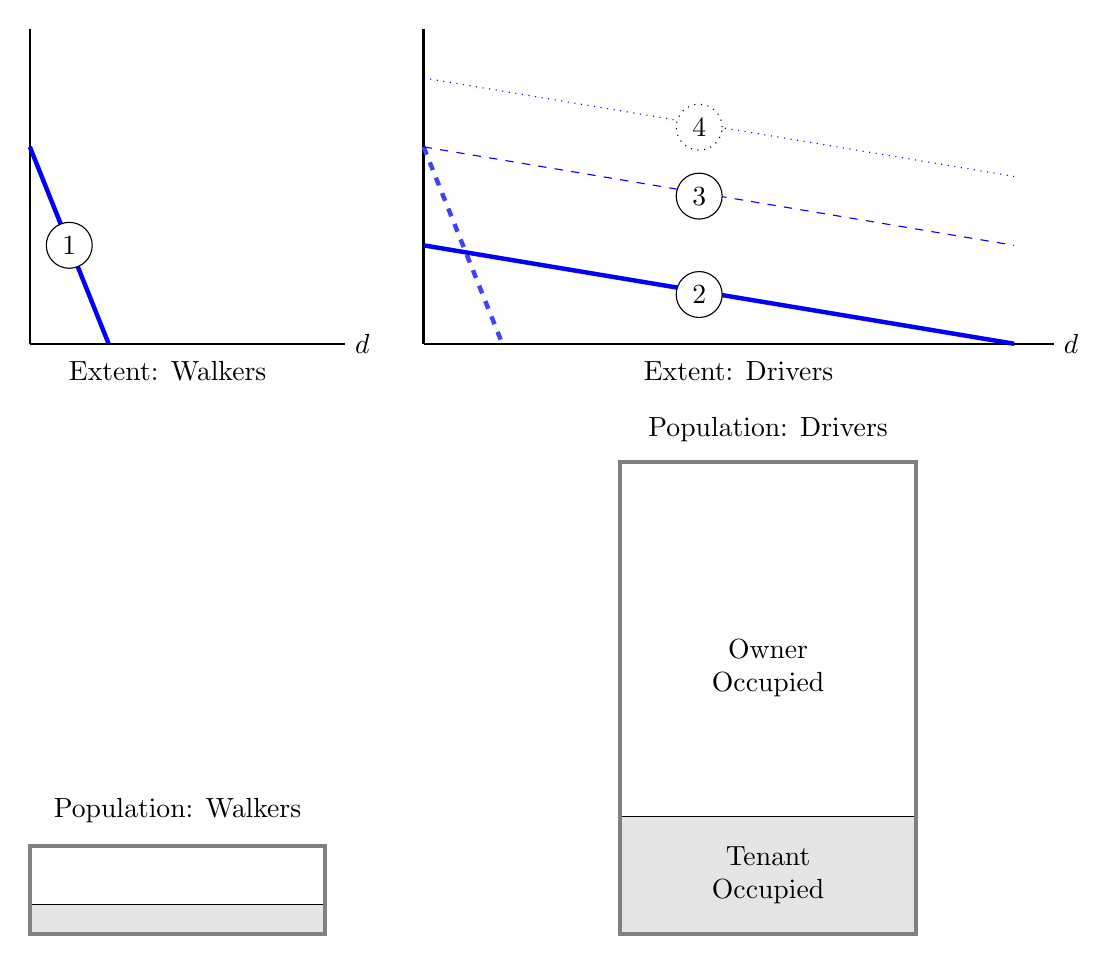
\begin{tikzpicture}[scale=.5]
% EXTENT  BEFORE
\draw[thick](0,0)--(0,8); %Y
\draw[thick](0,0)--(8,0)node[right]{$d$};
\node at (3.5,-.7){Extent: Walkers};
\draw[ultra thick, blue](0,5)--(2,0); 
\node[circle,draw=black, fill=white, inner sep=3pt,minimum size=10pt] (b) at (1,2.5) {1};

% POPULATION BEFORE
\begin{scope}[shift={(0, -15cm)},scale=1.5]%population
\draw [fill=gray!20,] (0,0) rectangle (5,.5); 
\draw[line width= .5mm, black!50] (0,0) rectangle (5,1.5);
\node at (2.5,2.1){Population: Walkers};
\end{scope}

% EXTENT AFTER
\begin{scope}[shift={(10cm, 0)}]
\draw[thick](0,0)--(0,8); %Y
\draw[thick](0,0)--(16,0)node[right]{$d$}; %X
\node at (8,-.7){Extent: Drivers};
\draw[ultra thick, blue!75, dashed](0,5)--(2,0);
\draw[ultra thick, blue](0,2.5)--(15,0);

\node[circle,draw=black, fill=white, inner sep=3pt,minimum size=10pt] (b) at (7,1.25) {2};

\draw[ blue, dashed](0,5)--(15,2.5);
\node[circle,draw=black, fill=white, inner sep=3pt,minimum size=10pt] (b) at (7,3.75) {3};

\draw[ blue, dotted](0,6.75)--(15,4.25);
\node[circle,draw=black, dotted,fill=white, inner sep=3pt,minimum size=10pt] (b) at (7,5.5) {4};
\end{scope}

% POPULATION AFTER
\begin{scope}[shift={(15, -15cm)},scale=1.5]%population
\draw [fill=gray!20,] (0,0) rectangle (5,2); 
\draw[line width= .5mm, black!50] (0,0) rectangle (5,8);
\node at (2.5,8.55){Population: Drivers};
\node at (2.5,4.5)
    [text width=2.4cm, align=center]
    {\baselineskip=20pt Owner Occupied};
%\node at (2,3.3)    [text width=2.4cm]    {\baselineskip=20pt Mortgaged};
\node at (2.5,1)
    [text width=2.4cm, align=center]
    {\baselineskip=20pt Tenant Occupied};
\end{scope}
\label{fig-rent-driving}
\end{tikzpicture}
\caption{Housing tenure post transportation revolution.}
\label{fig-transport-tenure}
\end{figure} 
 
%\input{fig_TransportCost.tex}

The transportation cost revolution brought about by the first street cars and later automobiles made much larger cities possible.  The average walking pace is 2.5 to 4 mph, and new transportation technologies raise this rate by a factor of between five and ten, increasing potential urban area by between twenty-five and one hundred times.   

% THIS IS INTERSTING K.  morgages: Effect of a finbancial instument on urban form!!  suburban flight, second half of the century

%Electric trolleys drew upon manufacturing technology that appeared only in the eighteen eighties and at first only in America. 

%As with other transportation revolutions, institutional as well as technological revolutions were necessary for the interurban phenomenon to succeed.  One such institutional revolution was the creation of the home mortgage in the eighteen eighties.  Another was the development of the public utility, a regulated monopoly, in the earlier twentieth. century.\footnote{https://faculty.washington.edu/jbs/itrans/charge20.htm} The automotive revolution was as important in its way as the coming of the railroads.

%The automobile in time established even more powerful synergies, but they weren’t present at the beginning.  Roads suitable for automobiles scarcely existed though new methods of paving utilizing macadam or concrete had recently been invented.  Furthermore, there was no good model in place for road construction.   Unlike the case with either light or heavy rail systems, the vehicles and the road itself were not part of the same corporate entity.       

%Once automotive ownership assumed certain proportions toward the close of the teens of the century, the automobile began to transform the landscape of America in an even more fundamental way than the streetcars had. 

%From the second decade of the twentieth century, the automobile in America has been linked with suburban flight, and when the growth of suburbs reached a crescendo early in the second half of the century, automobile ownership became the norm. 

% Because exurbs are already numerous and growing more so, they place considerable pressure on the Body Politic to ensure that fuel prices remain low, for if prices rise beyond a certain point the exurbanites will be forced to sell out, probably at ruinously low returns because few will choose to live in isolated areas without affordable transportation.  True, exurbs could conceivably be served by public transportation, but only at enormous cost per rider because the population densities are so low in the areas where they are located....

% That places the vast suburb dwelling public at risk and the exurbanites most of all.

Initially, rents fell at the centre and rose outside of the original city limits. Lower rents and cheaper suburban housing attract more workers, so that central rents and the land values they support  rise to the original levels and then, because the rising population makes the city more productive, beyond the original level. 

It  also affected social structure and left indelible marks on the form of cities developing at the time and after. In North America, with large amounts of land, it generated massive urban sprawl, but also made land available for a growing `middle class' of homeowners. This homeowning middle class became the dominant social formation in North 
American society. 

Ultimately the urban expansion generated congestion and rising transportation cost that began to limit urban growth, put upward pressure on  housing costs including transportation, and therefore downward pressure on middle-class effective incomes. Rising congestion costs steepen the rent profile and  reduce the net productivity of cities. Although the process is not a focus of this thesis it represents a relatively simple extension for later work.

\subsection{Class structure} \label{section-class-structure}
At the stage illustrated on the right  in Figure~\ref{fig-rent-driving},  %(Alonzo city suburbanized with owner occupiers) 
as a result of rapidly rising productivity, falling transportation costs, and large amounts of land with relatively low productivity, a new urban social system has emerged with a land-owning working class. 

The term \gls{class} is often used informally as if it refers straightforwardly to people who have different levels of wealth, but when economists talk about classes, they usually mean something slightly different. Economic classes are functionally defined:  by how they participate in production. Owners of labour participate by supplying their labour, for which they are paid a wage. Landowners own the land and receive rents for the use of their land in production. Owners of capital provide funds for starting and operating businesses, for which they receive profits.  There are three classes in this model and three kinds of income.  %It's because the surplus is differently distributed that different have different wealth levels. 

This emergence of a land owning working class is a recent phenomenon, and perhaps primarily a North American one. We are concerned in this thesis with whether may also be a passing stage.

America's economic transformation in the early 1800s was linked to dramatic changes in transportation networks. The construction of roads, canals, and railroads led to the expansion of markets, facilitated the movement of peoples, and altered the physical landscape. The later commuter transportation revolution further transformed cities and class structures.

\begin{figure}
\begin{center}
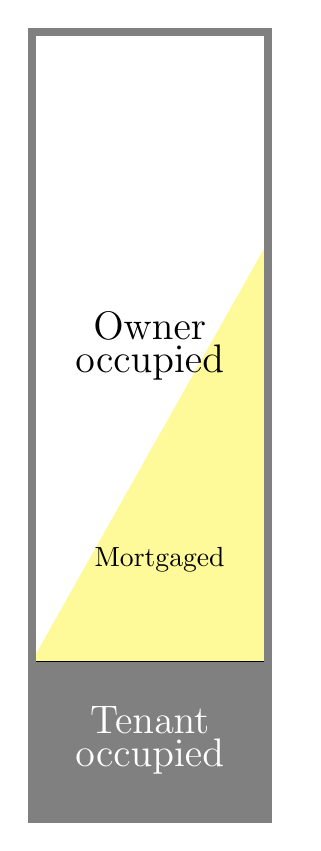
\begin{tikzpicture}{scale=.5}
\draw [fill=gray,] (0,0) rectangle (3,2); %TENANT
\draw [fill=yellow!40] (0,2)--(3,2)--(3,7.33); --cycle;% MORTGAGE %Calculation. 80\%owner, so  8 above the tenant line. 2/3*8=5.333. 5.333+2=
\draw[line width= 1mm, black!50] (0,0) rectangle (3,10);
\node at (1.5,6)
    [text width=2.4cm, align=center]
    {\baselineskip=20pt\Large Owner occupied};
\node at (2,3.3)
    [text width=2.4cm]
    {\baselineskip=20pt Mortgaged};
\node at (1.5,1)
    [text width=2.4cm, align=center, white]
    {\baselineskip=20pt\Large Tenant occupied};
% \caption{}
\end{tikzpicture}
\end{center}
\caption{Housing tenure and mortgaged share.}
\label{fig-mortgage-tenure}
\end{figure}


\section{Analysis list}

- why people hold onto baby boomer homes
- what happens with suburbanization
- speculative agent cycle- 
- pernicious cycle - lean into investment, rentals, lowered interst and increased supply actually amplify the problem
- pumps wealth out on the way up and on the way down


Potential interventions and systems shifts.. oasis cities..